% !TEX root = ../../main.tex

\section{The defective nature of MOFs}

\subsection{Types of crystal defects and their analogues in MOFs}

From a crystallographic point of view, defects can be described
as features which suspend the order of components in an ideally
regular lattice. The building blocks in the case of \glspl{MOF} can be either
individual atoms, molecules or other higher order \glspl{SBU}. 
Any change with leads to local breaking of symmetry with
respect to that original structure can be viewed as a defect.

With respect to dimensionality, defects can be described
as point defects, line defects (such as edge dislocations),
plane defects (such as grain boundaries or stacking faults) and bulk
defects (macroscopic voids, phase coexistence).
When it comes to point defects, we can broadly refer to several types:
\textbf{substitutional defects}, where an existing building unit is
replaced or transformed into another, \textbf{inclusion} or
\textbf{interstitial defects}, where a foreign component
or building block is included in the framework and \textbf{vacancy defects}
where one of the lattice sites is unoccupied.
In the context of \glspl{MOF}, the same general categories of defects
apply. However, due to the higher degrees of freedom available in
these compounds, a greater variety of potential crystal defects
can exist.

\textbf{Vacancy} defects are encountered through missing linker and
missing cluster defects. These analogues to Schottky defects
arise from the removal of one or several topological nodes or vertices.
In most cases, the charge neutrality of the framework
is maintained through coordination of available counterions or solvent
molecules, though changes in the oxidation state of the metal atoms
may also occur.

\textbf{Substitution} point defects are also highly common in \glspl{MOF}, as the
usual requirement for framework connectivity is the existence
of ``click groups'' on metal nodes and linkers. Any
molecule which fulfils the connectivity and size requirements may
be used, a property which has been exploited in the topological
approach to creating new 
\glspl{MOF}~\cite{burnettRecentAdvancesPorphyrinic2012,%
    liTopologicalAnalysisMetal2014,% 
    stockSynthesisMetalOrganicFrameworks2012}.
It also allows for \glspl{MOF} in which nodes or vertices are only partly
replaced with analogues to be created. This strategy has been
successfully employed to create mixed-linker or mixed-metal 
structures~\cite{buekenTacklingDefectConundrum2017,%
	dhakshinamoorthyMixedmetalMixedlinkerMetal2016}.
It should be noted that if the distribution of the substitutions takes
a homogenous pattern throughout the lattice, the structure may no
longer fall under the definition of a defect.

A special case of substitutional defects which are present in \glspl{MOF}
are mixed valence defects. When metals with multiple stable oxidation
states, such as \ce{Cu (I-II)}, \ce{Fe (II-III)} etc.\ are part of
the framework, a change in their oxidation state can occur. This has
been shown to be an integral part of copper paddlewheel and
iron trimesate containing \glspl{MOF}
~\cite{yoonControlledReducibilityMetalOrganic2010} and can even be
seen with the naked eye, as such defects have been shown
to give HKUST-1 its common blue colour~\cite{mullerDefectsColorCenters2017}.

\textbf{Inclusion}-type point defects are loosely applied to \glspl{MOF}.
As the definition describes an interstitial defect
to be an atom occupying an usually vacant space, all foreign
bodies occupying the available porosity of the \gls{MOF}, including
aforementioned counterions and solvents could be considered as
defects in the traditional crystallographic sense.
Introduction of nanoparticles such as metals or metal oxides
inside the pores is a more traditional view of such defects.
These have been shown to have beneficial
effects in catalytical
applications~\cite{falcaroApplicationMetalMetal2016, %
    schroderRutheniumNanoparticlesPorous2008}.

\begin{figure}[tb]
	\centering

	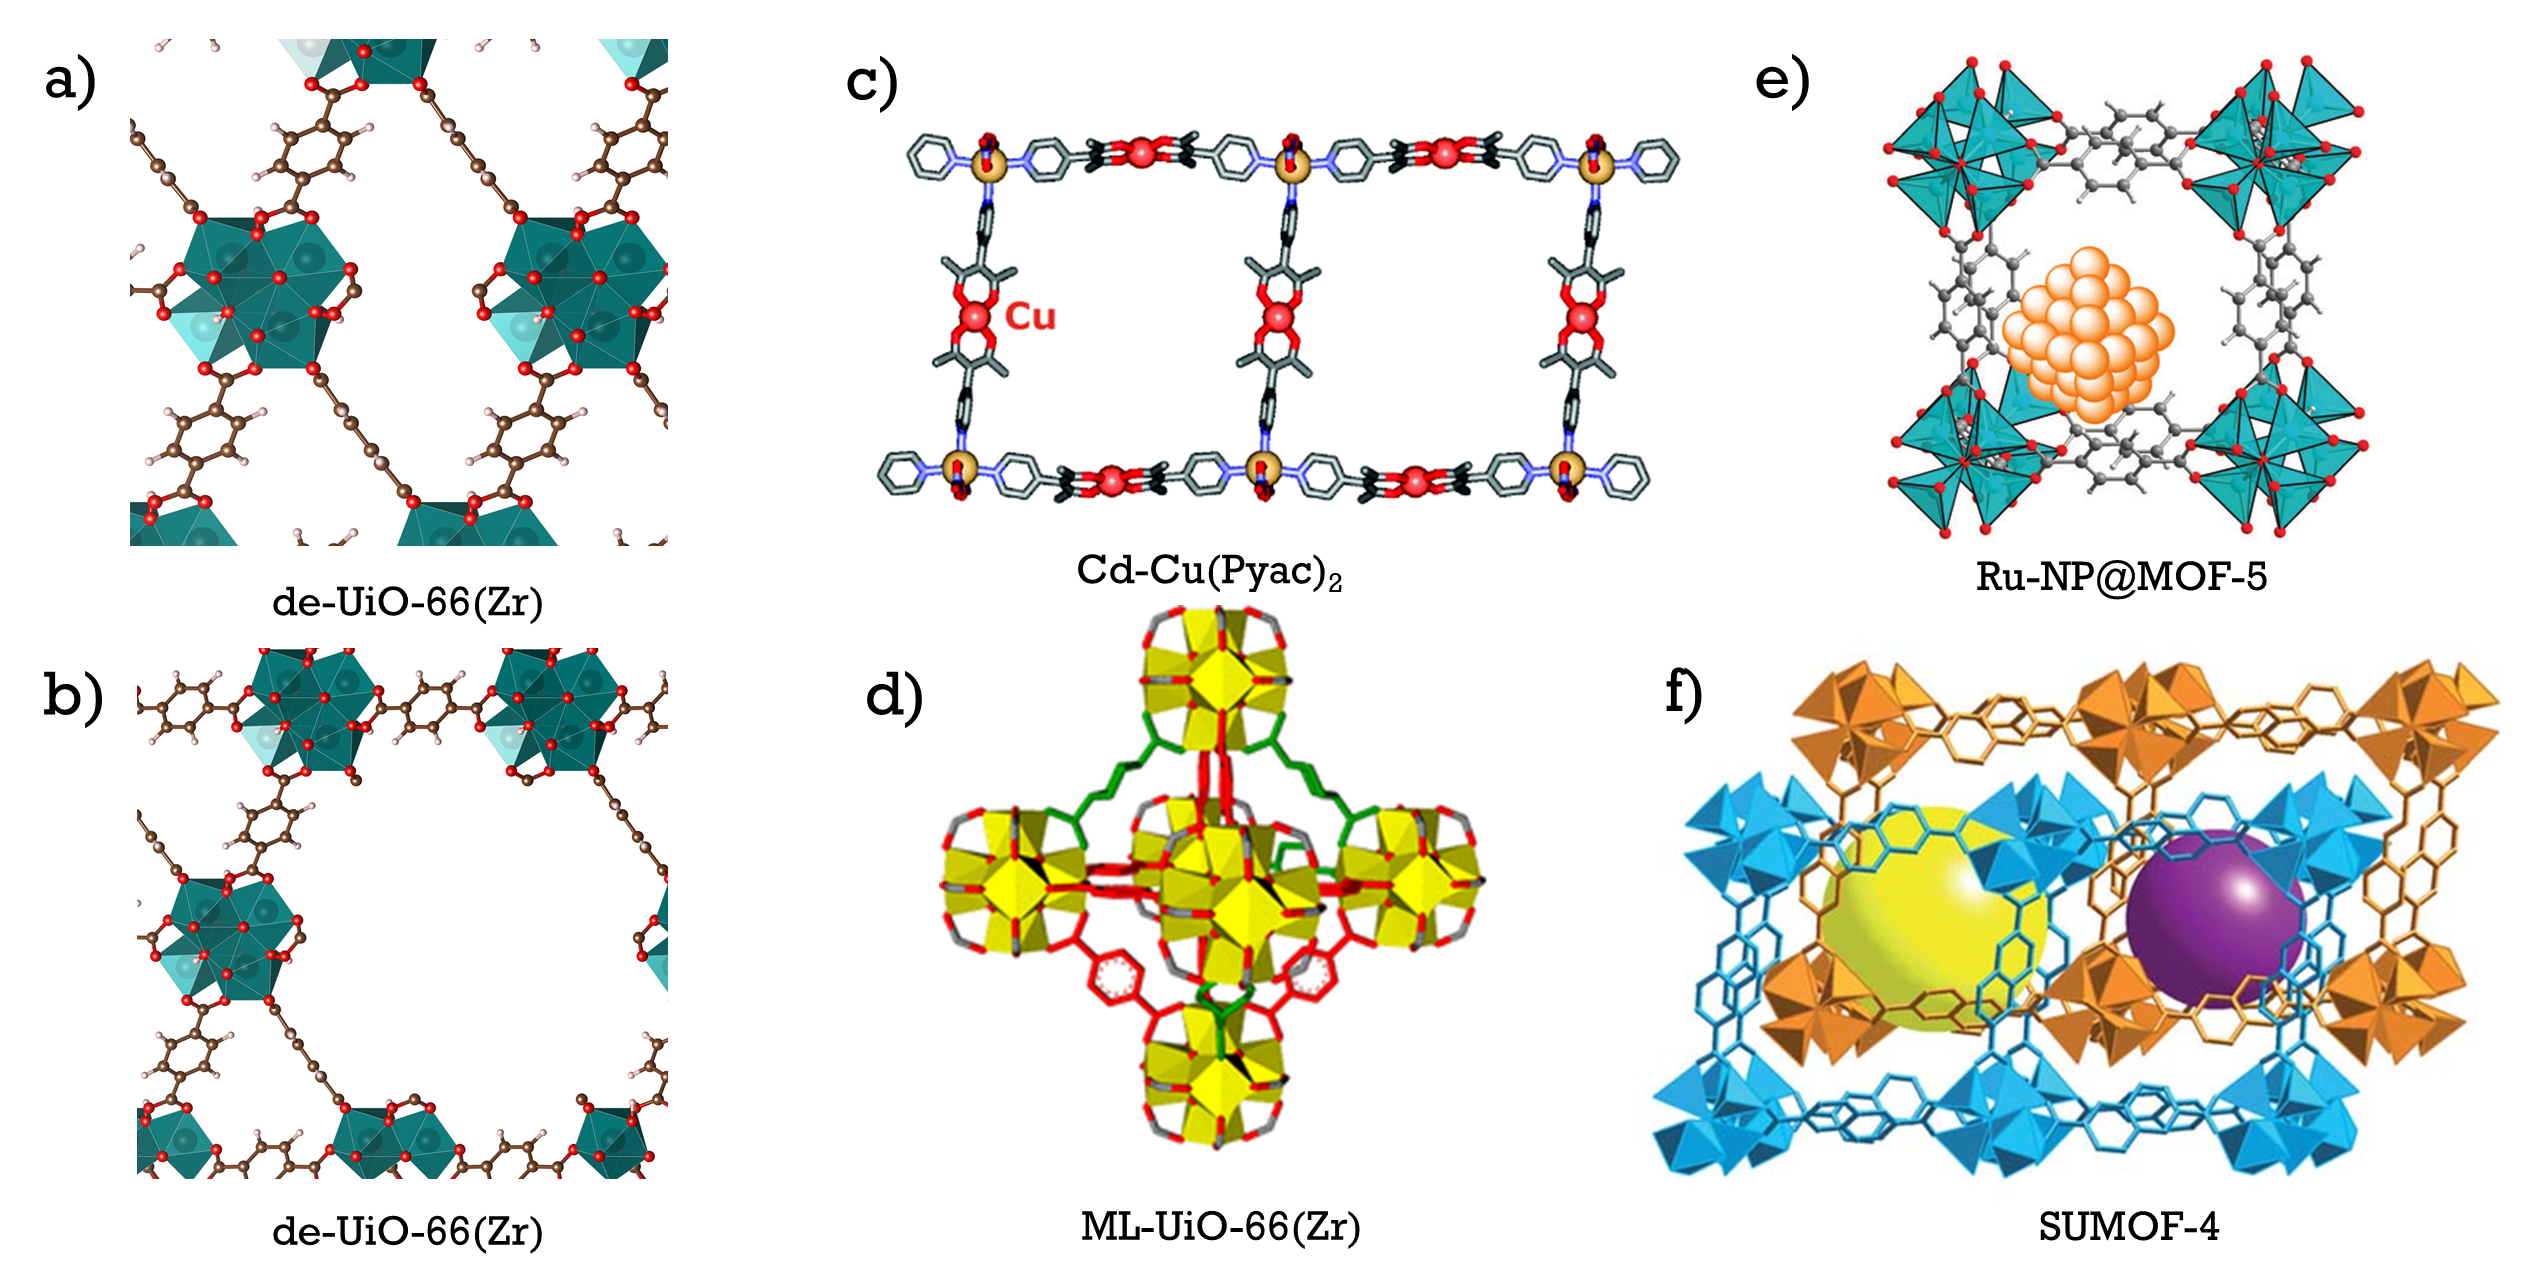
\includegraphics[width=\textwidth]{structures/defect-examples}
	\caption{
		Different types of defects as seen in \glspl{MOF}: 
		vacancy defects in the form of (a) missing linker and 
		(b) missing cluster substitutional defects such as
		(c) mixed linker~\cite{buekenTacklingDefectConundrum2017}
		and (d) mixed metal~\cite{vuongSynthesisEngineeringPorosity2013} \glspl{MOF} or defects 
		as created through (e) nanoparticles~\cite{schroderRutheniumNanoparticlesPorous2008}
		or (f) interpenetration~\cite{yaoInterpenetratedMetalOrganic2012}
	}%
	\label{def:fig:defect-types}
\end{figure}

A common feature of structured high porosity compounds is
interpenetration. While not a defect in the classical sense,
it has important effects on their 
properties~\cite{haldarInterpenetrationCoordinationPolymers2015}.
With a large enough pore size, a secondary lattice can form in the
pore voids of the primary one. This imposes a limit on the
common design strategy of isoreticular synthesis, but can
introduce new features such as better adsorption through
confinement, increase in active site count and even flexibility.

Finally, the surface of the \gls{MOF} can also be regarded as a
boundary or plane defect. The nature of the surface plays a role
in intra-particle interactions, important when considering
the agglomeration behaviour or inclusion of crystals in
a membrane~\cite{seminoMicroscopicModelMetal2016}.
The surface properties play a crucial role in \glspl{MOF} which 
are synthesised as thin 
films~\cite{gliemannEpitaxiallyGrownMetalorganic2012, %
	stassenUpdatedRoadmapIntegration2017}, where the nearly
2D materials are better defined by interfacial characteristics
than through bulk properties.
Crystal size effects on \gls{MOF} properties such as flexibility
can also be through of as a consequence of surface characteristics, 
more specifically of surface-to-volume ratio. When considering 
such soft materials~\cite{krauseEffectCrystalliteSize2018, %
	vanduyfhuysThermodynamicInsightStimuliresponsive2018}, it has
been shown that the flexible behaviour is highly influenced
by entropy barriers introduced by the surface.

\subsection{Consequences of defects}

The introduction of defects in the regular crystal lattice of metal
organic frameworks can have a dramatic impact on their properties.
In general, the following may occur:

\begin{itemize}
	\item the porosity of the structured is altered, increasing
	      in the case of vacancy defects and decreasing when bulky
	      substitutions or inclusions are made;
	\item interactions with adsorbed molecules change,
	      through the different pore environment encountered or
	      through the generation of coordinatively unsaturated
	      sites (CUS);
	\item the stability of the resulting structure is lower
	      than that of the parent \gls{MOF}, influencing bulk mechanical
	      and thermal properties.
	\item electronic properties can be changed which may
	      affect the optical electric or magnetic behaviour of the
	      material.
\end{itemize}

From a purely geometric point of view, the introduction of missing
linker or missing cluster defects leads to more voids in the structure,
increasing its porosity. It often results in a larger
specific surface area and pore volume and thus useful for applications
such as gas storage which depend only on the available surface or
capacity. Macro-scale void networks can also be desirable, as the 
better developed pore network has a large impact on the transport
properties of the compound, increasing diffusion rates. 

The inclusion of defects also changes the landscape of the pore
walls leading to different interactions with adsorbed molecules.
Charge balancing counterions, molecules capping defect sites,
functionalisations of substituted linkers or CUS can change the
chemistry of the pore, with specific interactions towards certain
adsorbates~\cite{dissegnaUsingWaterAdsorption2017}.
For example, adsorption of water on oxo-Zr \glspl{MOF}, has been seen to
be dominated by the percentage of defects. The pore filling step can
shift from high partial pressure (0.6 \(p/p_0\)) to much lower pressures
as seen in UiO-66~\cite{ghoshWaterAdsorptionUiO662014} and
MOF-801~\cite{choiRoleStructuralDefects2018}. Defect site adsorbed
molecules can also lead to cooperative phenomena,
such as the beneficial effect of defect-adsorbed water on the
catalysis of Fischer esterification~\cite{caratelliNatureActiveSites2017}.
or the \ce{CO2} capture on amine-grafted metal 
centers~\cite{mcdonaldCooperativeInsertionCO22015}.
Another example can be seen in \glspl{MOF} containing \ce{Fe} trimers,
such as MIL-127(Fe) or MIL-100(Fe) where heating or acid treatment
can induce a reduction of one of the iron atoms, generating
additional Lewis sites for catalysis~\cite{yoonControlledReducibilityMetalOrganic2010}
or providing CUS for cooperative binding of carbon monoxide through
a spin transition mechanism~\cite{reedSpinTransitionMechanism2017}.

Of course, defects are also problematic. Most metal organic frameworks
synthesised to date suffer from poor stability. Even if the material
is crystalline when solvated, the framework may not have
enough structural stability to be able to sustain itself when fully
evacuated. The activation process itself can lead to framework
collapse, due to the forces encountered in guest removal, necessitating
complex activation processes, such as supercritical drying or
preliminary solvent exchange. After activation, the metal-ligand bond
is susceptible to attack by adsorbed species. Here, defects in the framework
have been shown to play a major role in its stability (or lack
thereof)~\cite{burtchWaterStabilityAdsorption2014}.
Copper paddlewheel containing structures are particularly vulnerable to
such attack~\cite{alvarezStructureStabilityHKUST12017}.

Finally, several completely different phenomena may emerge through
the introduction of defects. Optical properties such as colour
centers and induced luminescence~\cite{mullerDefectsColorCenters2017},
changes in thermal conductivity or induced magnetic properties
such as ferromagnetism~\cite{shenOriginLongRangeFerromagnetic2012}
have been shown to be a consequence of the presence of defects.

\subsection{Defect engineering of MOFs}

Since defects introduce another degree of freedom
for controlling the properties of metal organic frameworks, the
study of their formation can lead to new methods of tuning
a material towards a desired application.
There are two major pathways of introducing defects, through
control of the structure during synthesis or through post-synthetic
methods~\cite{fangDefectEngineeredMetalOrganicFrameworks2015}.

For defect generation during synthesis, the so called
``solid solution'' approach is to mix several types of
building blocks together, be it multiple linkers or
metallic nodes. Mixing functionalised versions of linkers
leads to the creation of partially-substituted \glspl{MOF}.
Mixed valency frameworks can also be synthesised through
this method, as can be seen in the replacement of up to 32\% of the
linker in the framework in the ruthenium HKUST-1
analogue with a defect-generating
linker~\cite{zhangRutheniumMetalOrganicFrameworks2016}.
The commonly used method of improving crystalinity and
particle size of modulator-assisted
synthesis~\cite{schaateModulatedSynthesisZrBased2011} has been shown
by~\citeauthor{shearerDefectEngineeringTuning2016}
to be a reliable method of introducing
defects~\cite{shearerDefectEngineeringTuning2016}.
The modulators act as capping agents and occupy metal coordination sites.

Post-synthetic methods are also widely employed for defect
generation. Through acid treatment of the previously mentioned
MIL-100(Fe), cleavage of one of the \ce{Fe-O} bonds can be
induced, with a protonation of the carboxylic linker and the
generation of a CUS.~\cite{vermoorteleTuningCatalyticPerformance2012}
Thermal treatment can achieve the same results, with weakly coordinated
molecules removed to expose metal CUS or even \textit{in situ}
linker decomposition~\cite{gadipelliPostsynthesisAnnealingMOF52014}.
Ligand exchange has also been shown to be achievable post-synthetically,
~\cite{shearerFunctionalizingDefectsPostsynthetic2016} through the
replacement of existing linkers, capping agents or even induce
structural ``healing''. Finally, the linkers are still available 
for organic reactions which can transform a part of them into
functionalised versions, as seen in the nitration of the 
terephtalate linker in MIL-101~\cite{berntDirectCovalentPostsynthetic2011}.

\subsection{The propensity of UiO-66(Zr) for defect generation}

The UiO-66(Zr) \gls{MOF} and its derivatives are well known due to
their thermal and chemical stability~\cite{cavkaNewZirconiumInorganic2008}.
It is composed of \ce{[Zr6O4(OH)4]^12+} clusters
(seen in \autoref{defects:fig:uio66-cluster}) which are connected
via \gls{BDC} linkers to form a face-centred cubic
framework. Due to its exceptional stability among \glspl{MOF}, it has been the
focus of much research, where it has shown
promise~\cite{wiersumEvaluationUiO66GasBased2011} in use for gas
adsorption and catalytic applications.

The synthesis of many functional derivatives of UiO-66,
through the use of different struts of nodes has been a stepping 
stone towards obtaining mixed-linker and mixed-metal materials, 
either thorough the solid solution or post-synthesis modification
approach~\cite{kimPostsyntheticLigandExchange2012}.
It has also been used as a support for nanoparticles, such
as palladium~\cite{shenHighlyDispersedPalladium2013}
or platinum~\cite{oienProbingReactivePlatinum2015}.

However, UiO-66 is particularly adept is in its ability to support
vacancy defects. Due to the stability of the metal-oxygen bond, and the
high linker to metal ratio, the UiO family of \glspl{MOF} can tolerate
a high degree of defectivity in their structure, which manifests through
either missing linker
(\autoref{defects:fig:uio66-defect-linker}) or missing
cluster (\autoref{defects:fig:uio66-defect-cluster}) defects.
Ever since the discovery of a number of
defects in the pristine material through neutron powder diffraction
methods~\cite{wuUnusualHighlyTunable2013} and the theoretical
basis laid down by~\citet{cliffeCorrelatedDefectNanoregions2014}
for the existence of correlated defective nanodomains where the
existence of a vacancy induces defect formation in neighbouring
sites, this \gls{MOF} became a prototypical framework for the study of
such defects.
The modulated synthesis approach, initially used as
a means of creating novel topologies and controlling crystal
size~\cite{guillermZirconiumMethacrylateOxocluster2010}
has been remarkably successful in obtaining defective versions
of UiO-66(Zr)~\cite{shearerDefectEngineeringTuning2016}.
Post-synthetic methods such as ligand
exchange~\cite{shearerFunctionalizingDefectsPostsynthetic2016},
temperature-induced dehydroxilation of the zirconium
cluster~\cite{valenzanoDisclosingComplexStructure2011} and
thermal removal of one of the linkers in a mixed-linker
variant~\cite{buekenTacklingDefectConundrum2017} have been
similarly adept in obtaining voids in the structure.
More recently, the interplay between the 
defective nature of UiO-66 and the mechanism of 
post-synthesis linker exchange~\cite{taddeiPostsyntheticLigandExchange2018}
has been put into the limelight.


\begin{figure}[tb]
	\centering

	\begin{subfigure}[b]{0.3\linewidth}
		\parbox[c]{0.15\linewidth}{\caption{}%
			\label{defects:fig:uio66-cluster}}%
		\parbox[b]{0.85\linewidth}{%
			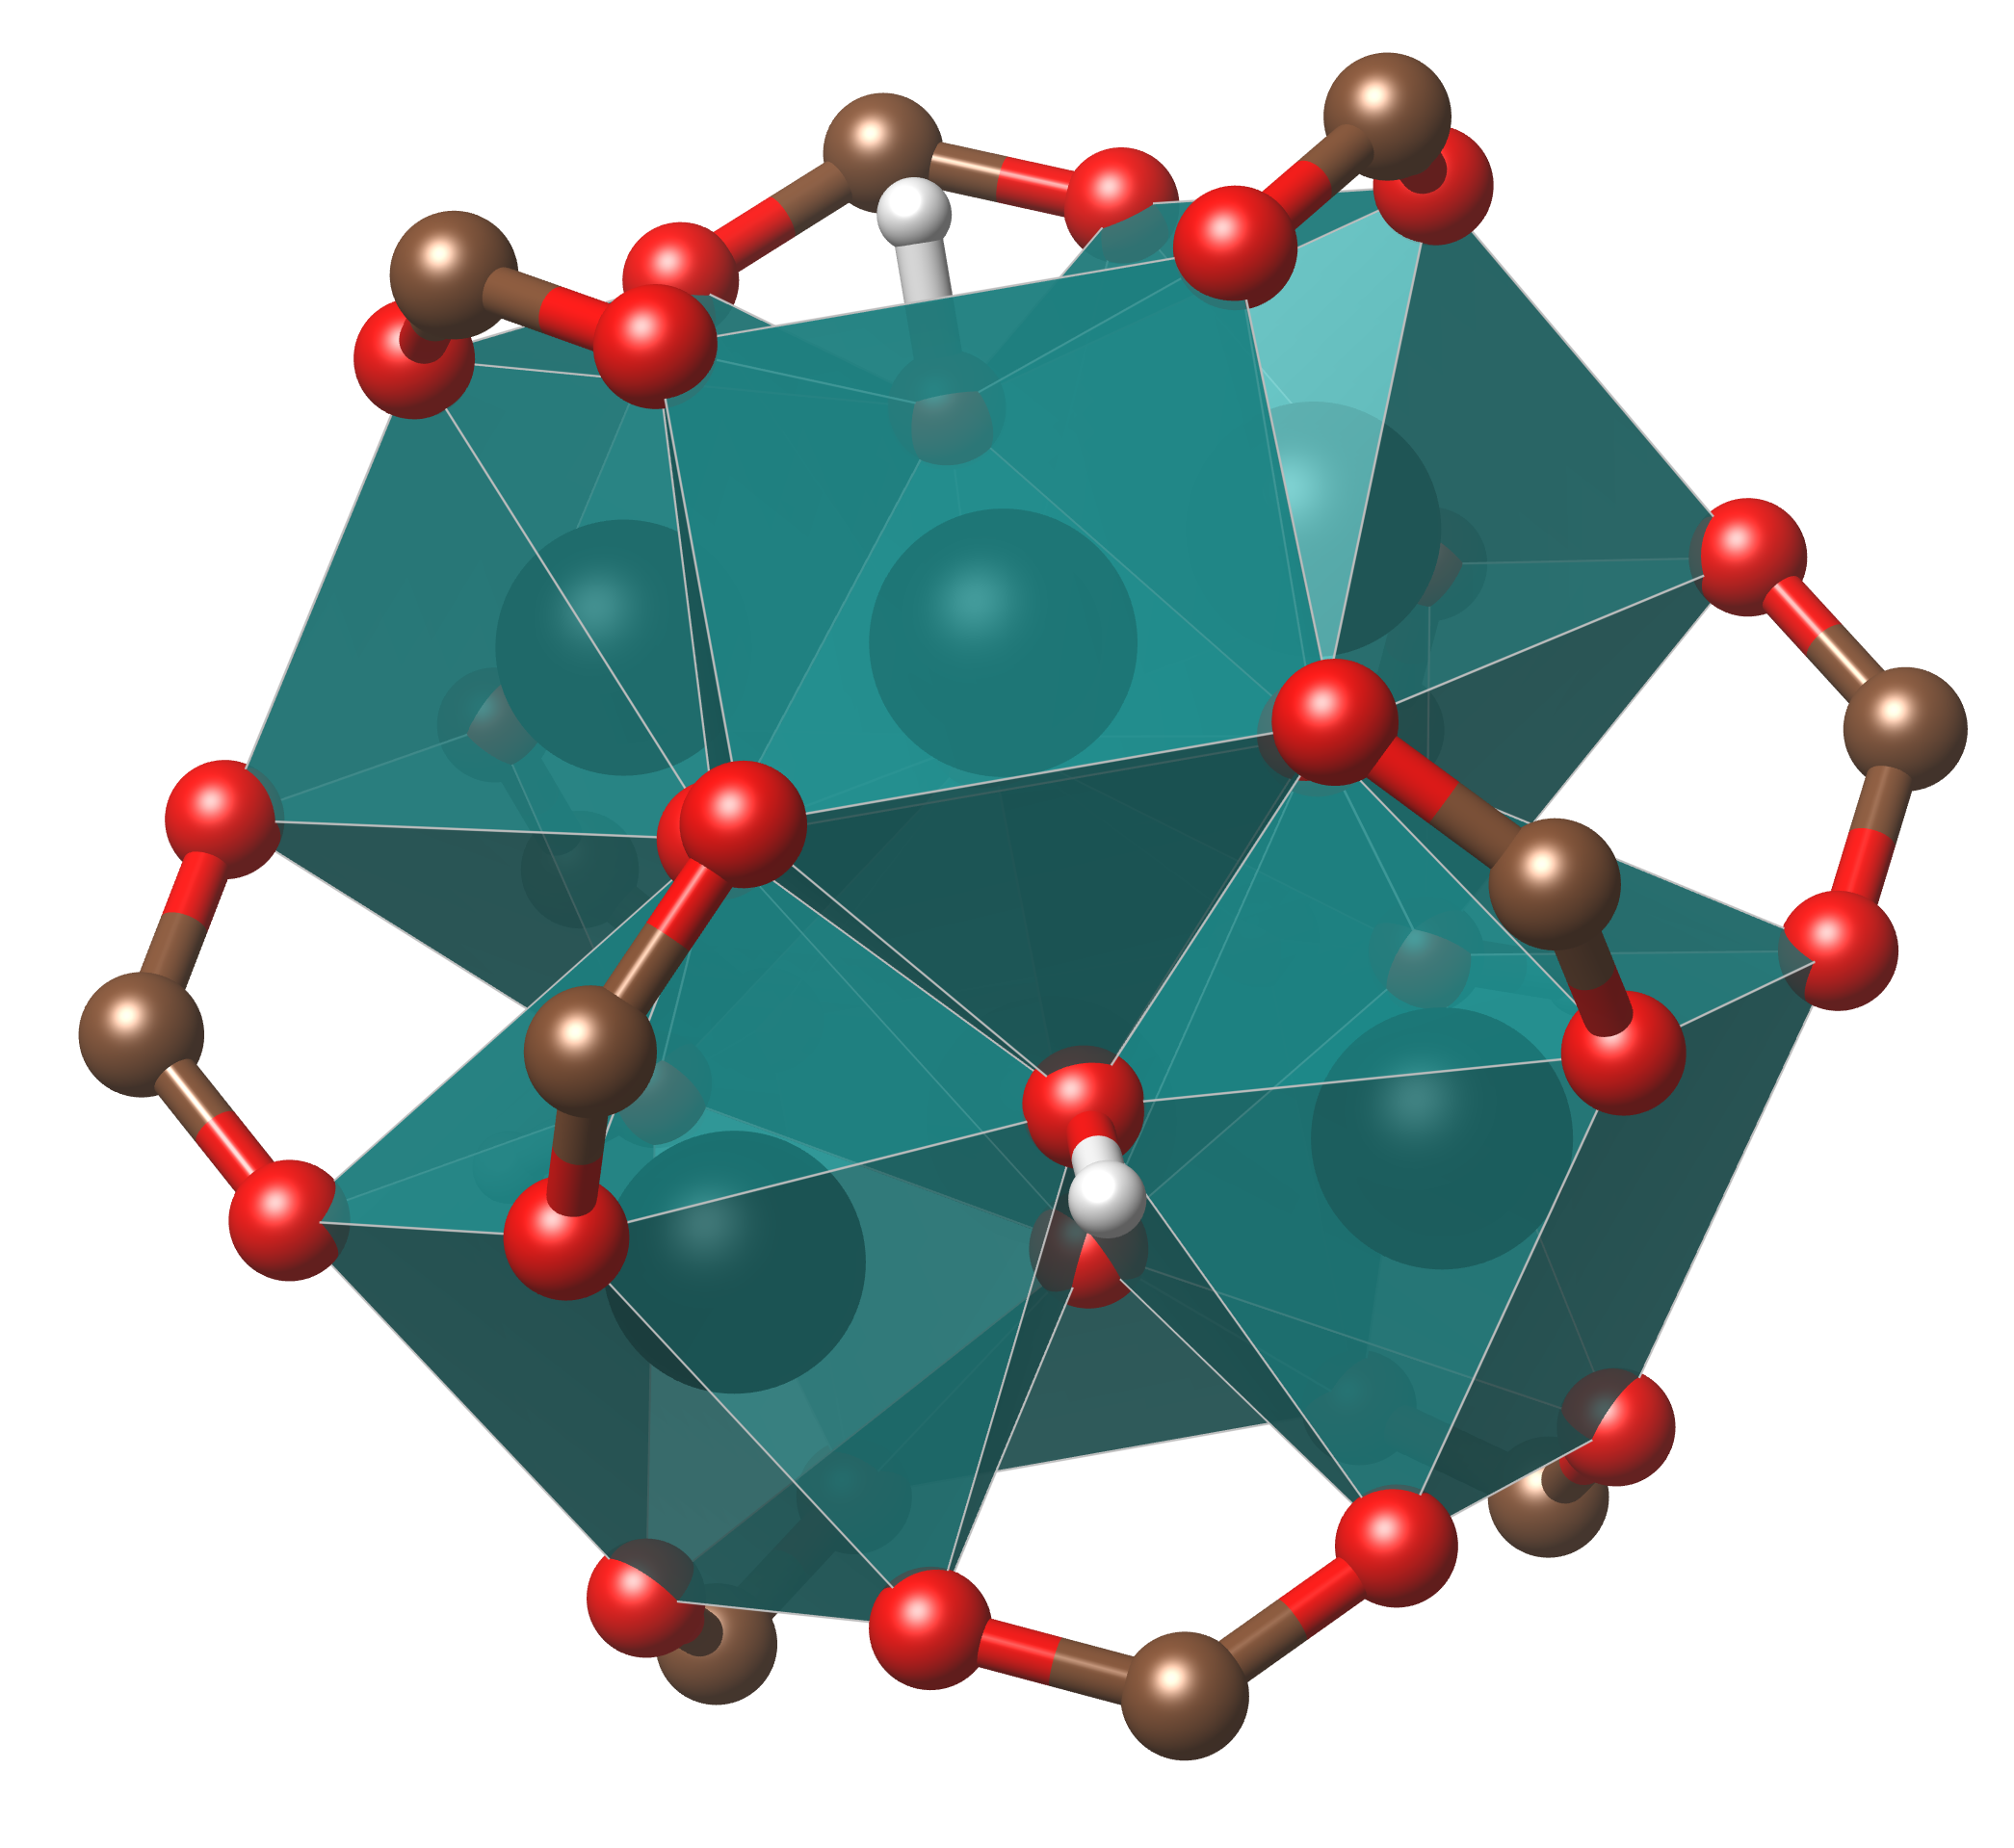
\includegraphics[width=\linewidth]{structures/uio66-cluster}%
		}%
	\end{subfigure}
	\begin{subfigure}[b]{0.3\linewidth}
		\parbox[c]{0.15\linewidth}{\caption{}%
			\label{defects:fig:uio66-defect-linker}}%
		\parbox[b]{0.85\linewidth}{%
			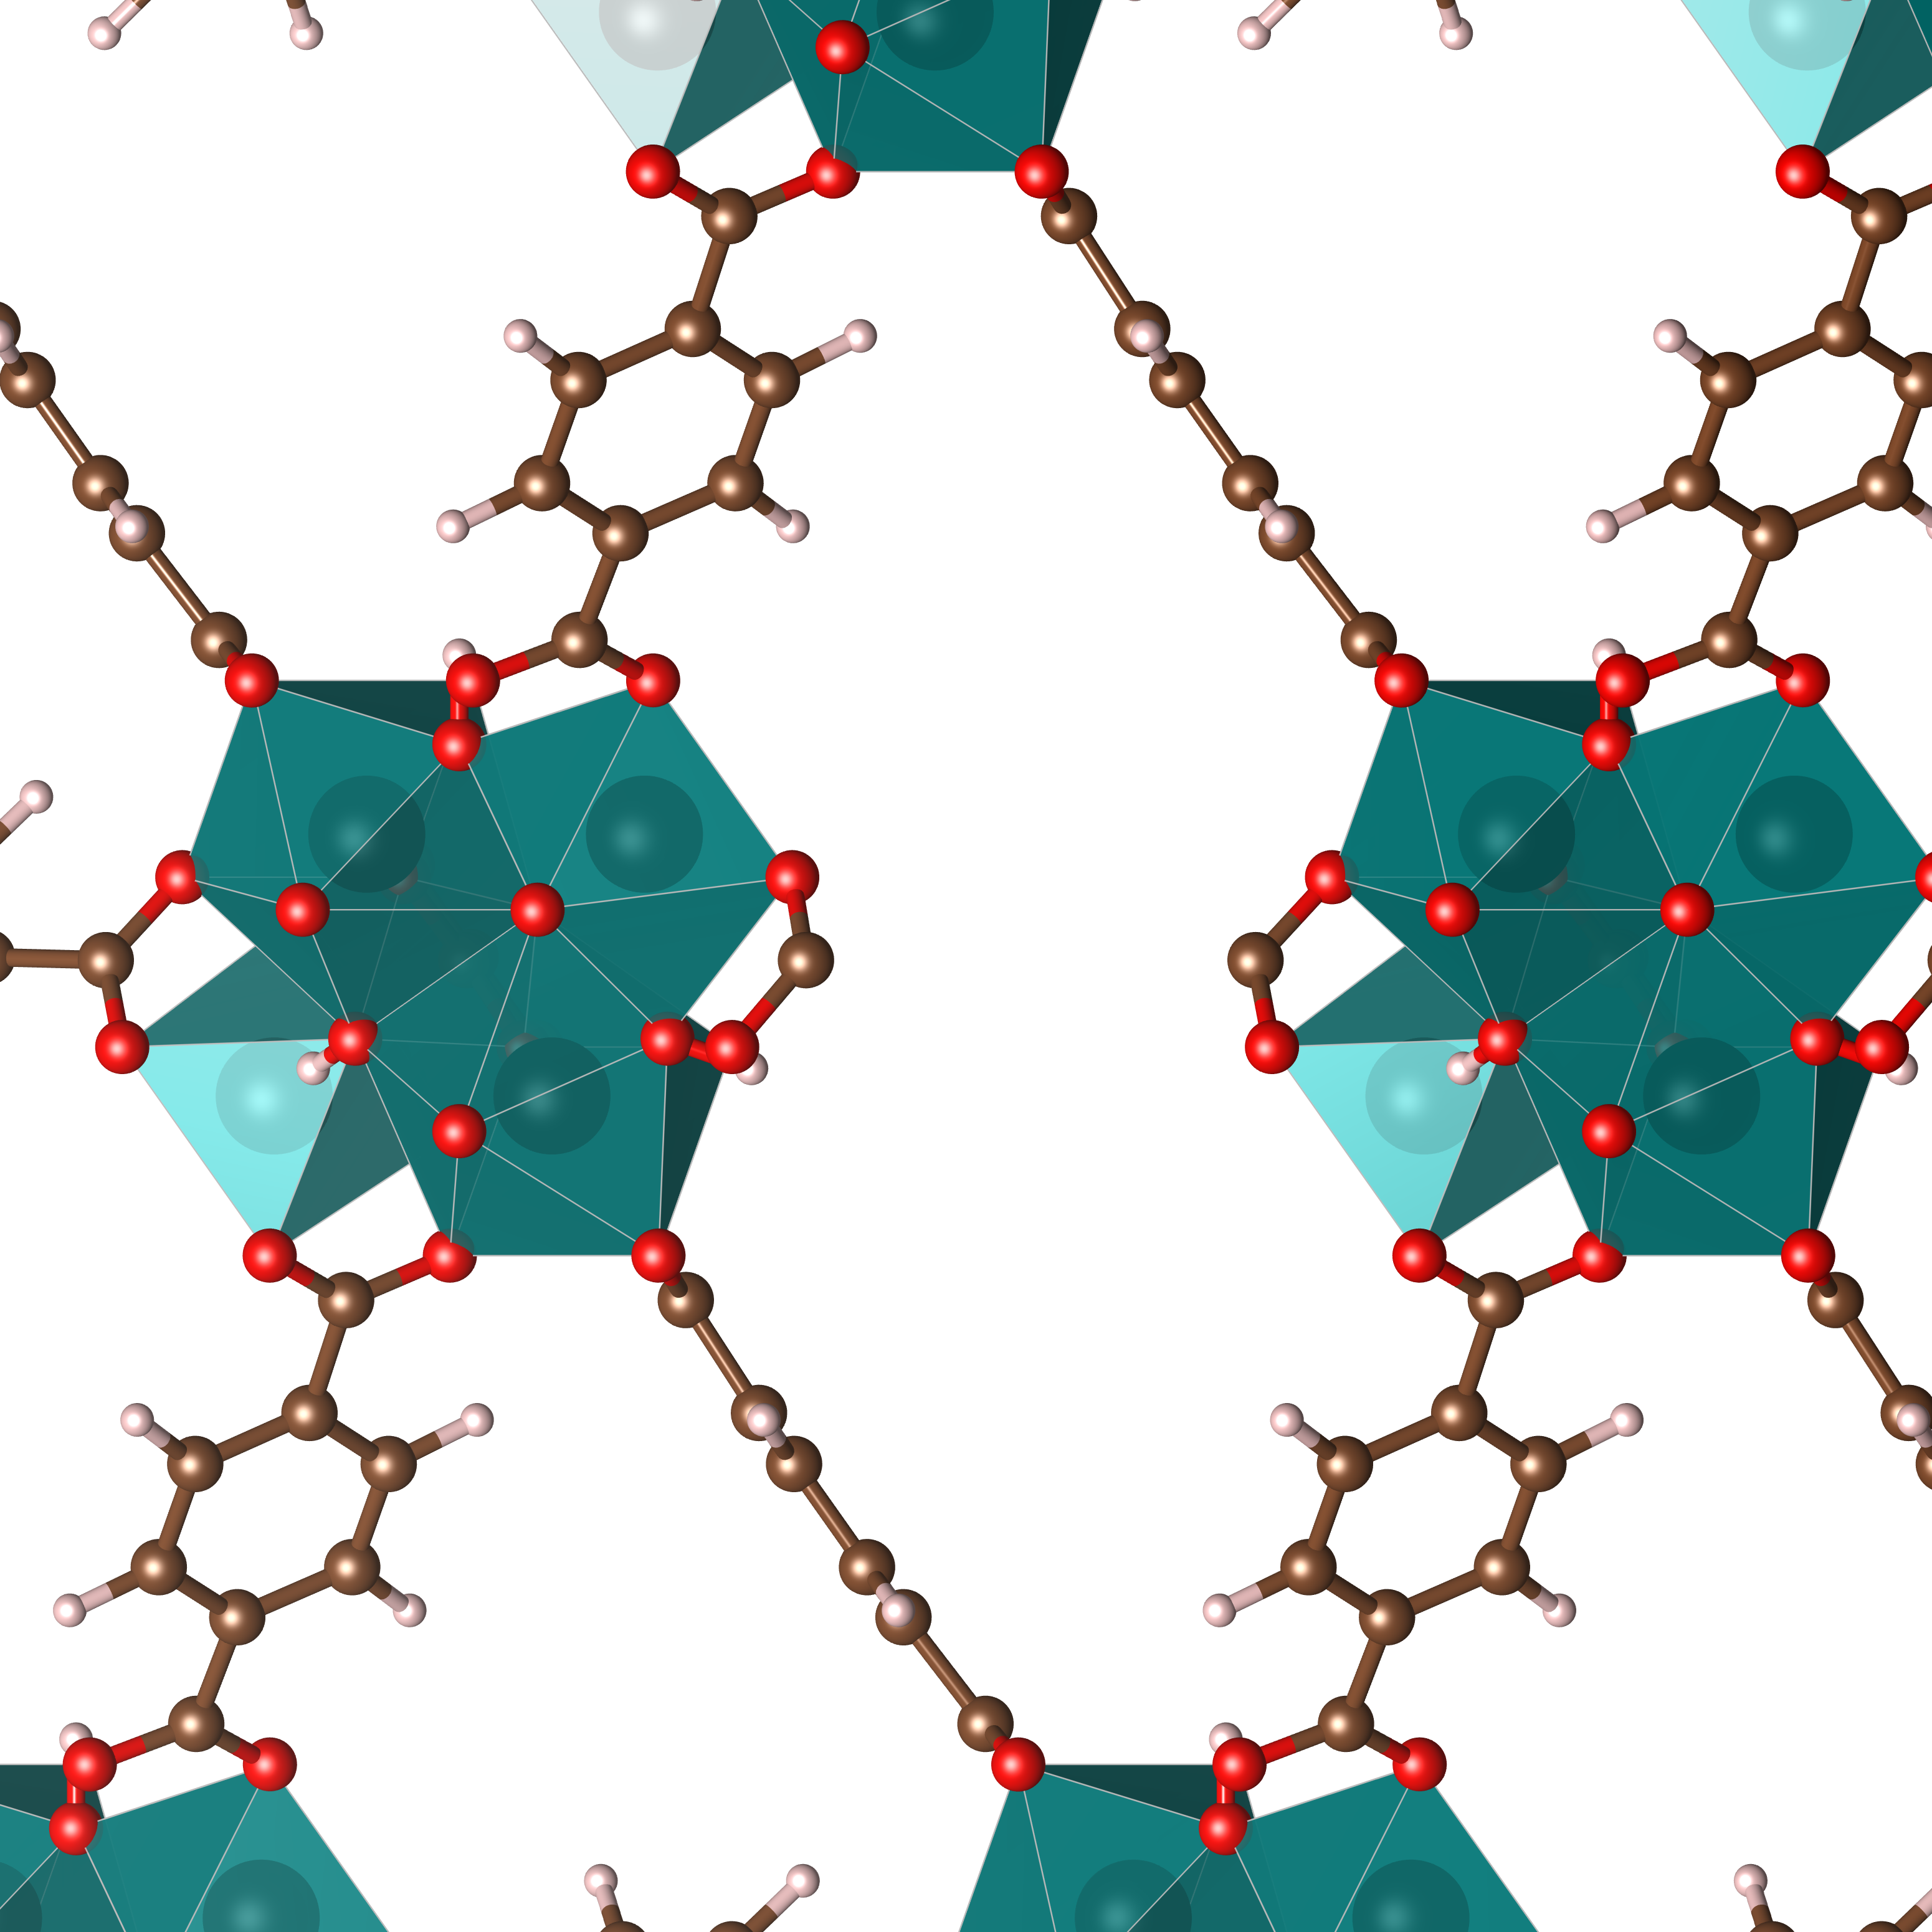
\includegraphics[width=\linewidth]{structures/uio66-defect-linker}%
		}%
	\end{subfigure}
	\begin{subfigure}[b]{0.3\linewidth}
		\parbox[c]{0.15\linewidth}{\caption{}%
			\label{defects:fig:uio66-defect-cluster}}%
		\parbox[b]{0.85\linewidth}{%
			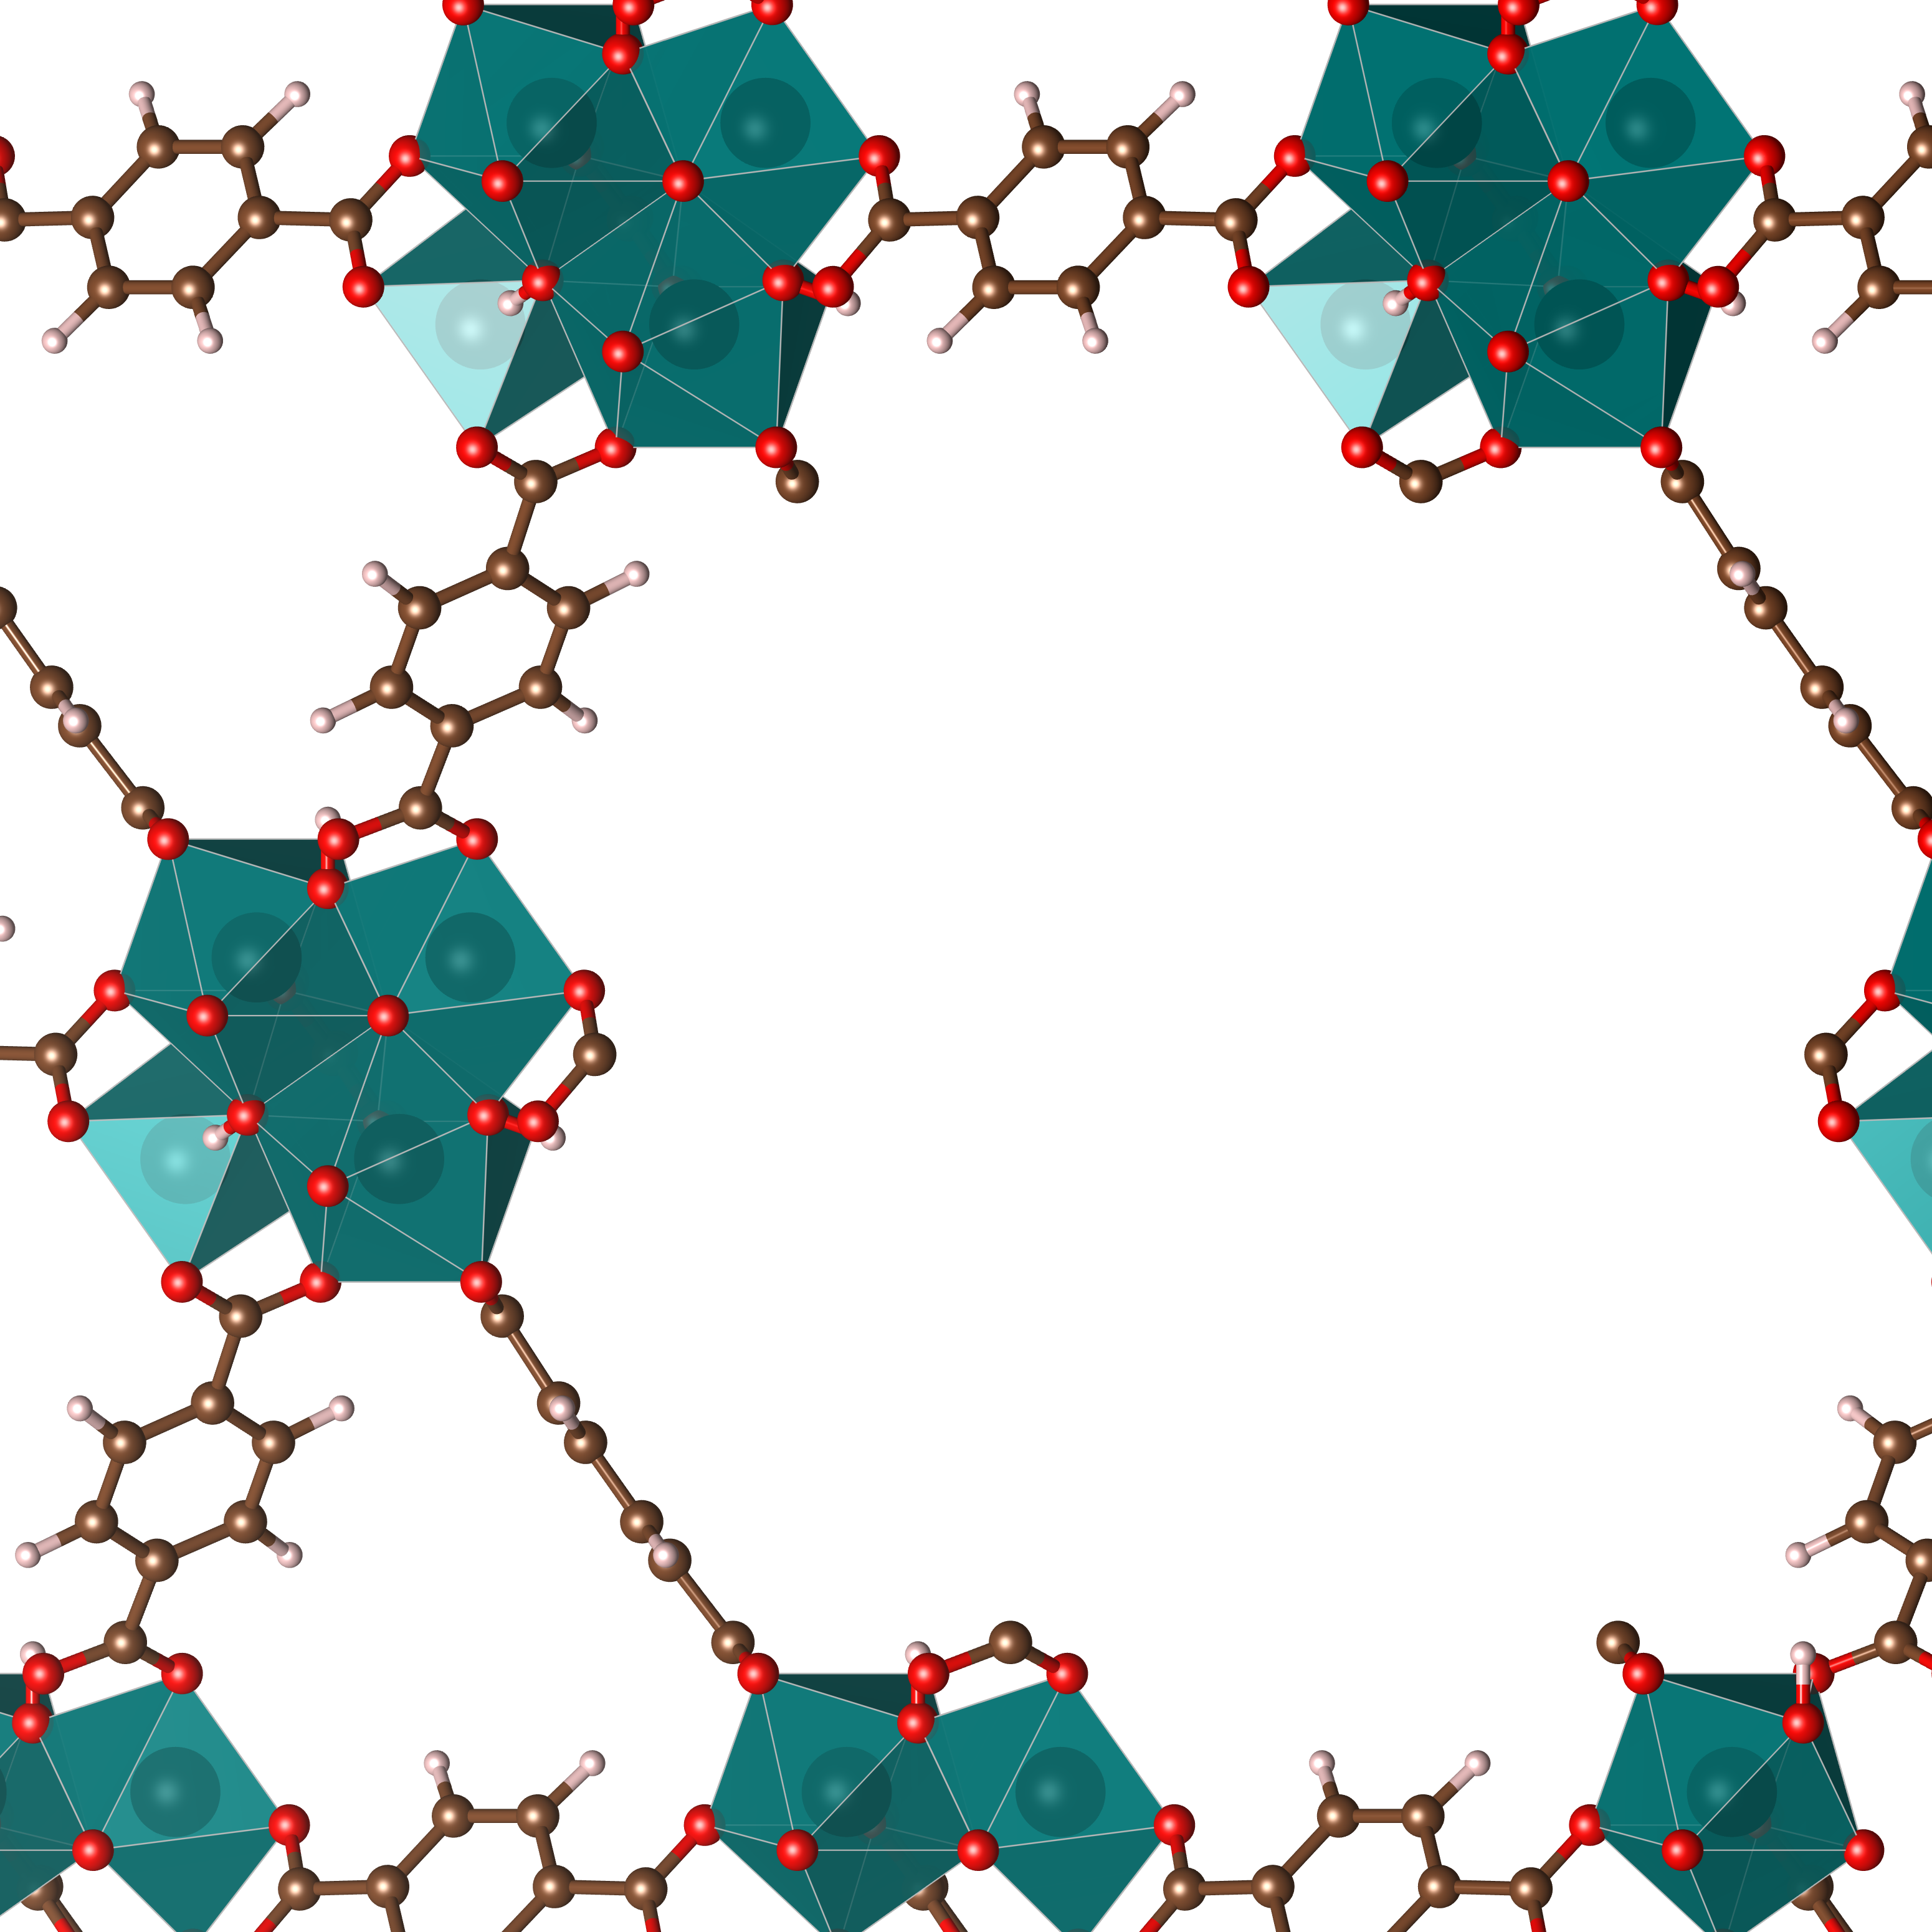
\includegraphics[width=\linewidth]{structures/uio66-defect-cluster}%
		}%
	\end{subfigure}

	\caption{(a) The 12-coordinated Zr cluster in UiO-66(Zr)
		which connects with benzene dicarboxilate (BDC) linkers.
		Two prototypical defect types are shown (b) a missing
		linker defect and (c) a missing cluster defect. Zirconium
		octahedra are represented in turquoise, oxygen in red,
		carbon in brown and hydrogen in white.}%
	\label{defects:fig:uio66}

\end{figure}

In these defects, the metal sites are almost always capped,
with monoacids such as formate and acetate, water, hydroxyl groups
or other counterions being able
to assume the role of capping agent. It has been shown
by~\citeauthor{thorntonDefectsMetalOrganic2016} that the influence
of such defects on the adsorption properties depend not only
on their position, but also on these capping
agents~\cite{thorntonDefectsMetalOrganic2016}. 

Such vacancy defects prove to be useful for generating Lewis
sites for catalytic application, as can be seen in the 
4-fold increase in conversion in citronellar cyclization or
the increase in 4-tert-butylcyclohexanone reduction from 
5--7\% to almost 90\%~\cite{vermoorteleSynthesisModulationTool2013}.
They are also useful for gas separation, as they can increase the 
interaction towards a component of the mixture, seen for example
on the increased efficiency of \ce{CO2 / N2}
separation~\cite{thorntonDefectsMetalOrganic2016}.

It can therefore be concluded that vacancy defects are a fundamental 
characteristic of this \gls{MOF}, with wide-ranging effects in its 
properties.
As such, it is desirable to have methods to generate and control
them. In the following pages, we examine a tertiary method 
for vacancy defect generation: leaching in solvent
solution, a method which has been previously shown to be applicable 
to other \glspl{MOF}~\cite{tuOrderedVacanciesTheir2014}.

